\documentclass[conference]{IEEEtran}
\IEEEoverridecommandlockouts
% The preceding line is only needed to identify funding in the first footnote. If that is unneeded, please comment it out.

\usepackage{amsmath}
\usepackage{todonotes}
\usepackage{algorithm}
\usepackage[noend]{algpseudocode}
\usepackage{cite}
\usepackage{amsmath,amssymb,amsfonts}
\usepackage{algorithmic}
\usepackage{graphicx}
\usepackage{textcomp}
\usepackage{xcolor}
\def\BibTeX{{\rm B\kern-.05em{\sc i\kern-.025em b}\kern-.08em
    T\kern-.1667em\lower.7ex\hbox{E}\kern-.125emX}}
    
\usepackage{atbegshi}% http://ctan.org/pkg/atbegshi
\AtBeginDocument{\AtBeginShipoutNext{\AtBeginShipoutDiscard}}


\begin{document}

\title{ Application Note: $\mu$Polar \-- An Interactive 2D Visualization Tool for  Microfluidics and  Microscopic Time Series Images }

% \author{\IEEEauthorblockN{1\textsuperscript{st} Mehran Ghafari}
% \IEEEauthorblockA{\textit{SimCenter, Dept. Computer Science and Engineering} \\
% \textit{University of Tennessee, Chattanooga, USA}\\
% ryg668@mocs.utc.edu}
% \and
% \IEEEauthorblockN{2\textsuperscript{nd} Hao-Bo Guo}
% \IEEEauthorblockA{\textit{SimCenter, Dept. Computer Science and Engineering} \\
% \textit{University of Tennessee, Chattanooga, USA}\\
% haobo-guo03@utc.edu}
% \and
% \IEEEauthorblockN{3\textsuperscript{rd} Weiwei Dang}
% \IEEEauthorblockA{\textit{Dept. Molecular and Human Genetics, Huffington Center on Aging}\\
% \textit{Baylor College of Medicine, Houston, USA}\\
% Weiwei.Dang@bcm.edu}
% \and
% \IEEEauthorblockN{4\textsuperscript{th} Hong Qin}
% \IEEEauthorblockA{\textit{SimCenter, Dept. Computer Science and Engineering}\\
% {Dept. Biology, Geology and Enviromental Science} \\
% \textit{University of Tennessee, Chattanooga, USA}\\
% hong-qin@utc.edu}
% }

\maketitle

\begin{abstract}
Microfluidics-based microscopy is becoming an increasingly popular research tool to monitor cellular events in biomedical research. One such application is the high-throughput analysis of dividing yeast cells. It is challenging to visualize and interpret the data gathered through microfluidics-based microscopy. Here, we developed a circular plotting method, $\mu$Plot, to visualize cell movements and cellular division events at hundreds of time points. Our method is interactive and easy to use. We demonstrated the utility of our method to describe the events of dividing yeast cells. Our method could be potentially applied to other types of microfluidic devices. This software is implemented in an R package $\mu$Polar \ available through GitHub. 
\end{abstract}


\begin{IEEEkeywords}
microfluidics image, Data, Visualization, plot 
\end{IEEEkeywords}

\section{Introduction}
 
The biological processes of cell lineage family tree that deployed in spatial and temporal are essential in the biomedical field including research, medicine and diagnosis a variety of diseases. Thus, quantitative analysis of cell behavior constructed on lineage tree tagged with appropriate measurements for the individual cell is the imperative basis for understanding the dynamics and structure of organisms \cite{r2.6}. Comprehensive and detailed information considering cell locality position, pathway, nucleus, formation, dissection, replicative and chronological lifespan can potentially be concluded from images using a combination of manual and automatic visualization tools \cite{r2.7}. Having an automatic tool that collects microscopic images and generates interactive visualization of the cell family tree with a quantitative comparison of cells would be a great requisite for many applications.

In the recent decade, crucial breakthroughs have been created and developed in the microscopy imaging of live-cell mechanisms such as fluorescent protein labeling, selective plane illumination microscopy (SPIM) and multiphoton laser scanning microscopy (MLSM)\cite{r2.7,r2.8,r2.9}. Concurrently, many image processing algorithms have been developed for cell segmentation (e.g, semantic and instance), tracking and quantitative analysis \cite{r2.10}.

Visualization can offer an efficient path to study the data obtained from live-cell imaging including high dimensional biological data. However, it has not adequately been developed in time-lapse microscopic images with interactive visualization. In other words, there is a knowledgeable gap between some biology areas and suitable visualization tools, in particular, visualizing the dynamic development of cells and lifespan. Furthermore, many of the experimental results from these microscopic images are based on numerical numbers which require expertise to verify the validation of the outcome. 

Microfluidics device is an ultra-small structure with microfluid channels offer faster and reliable results in comparison to traditional methods \cite {r2.1,r2.2}. Duo to their functionality, microscale or nanoscale dimension, they can be used in many applications such as drug delivery, cell monitoring, cell division, virus inspection and so on \cite{r2.3,r2.4}. Time-lapse microfluidics images amplify biologists ability to experimentally image live-cell during the developing progress \cite{r3}. Recently, a new network model of cellular aging was proposed based on the cellular aging process of yeast cells \cite{ref4.2}. For instance, Jo et al. \cite{\r13} investigated the high-throughput analysis of dividing yeast cells using microfluidic devices. 

Cell division enumeration is a budding yeast process that is one of the essential factors in aging where single mother cells can be accomplished before inactivation, also known as replicative lifespan (RLS). Determining the lifespan of cells is a time-consuming process and in many cases is based on manual operation, such as cell microdissection \cite{ref08}. Accordingly, visualization of cell growth and division potentially can offer a great point of view to estimate RLS of cells (e.g, yeast) with would have an effective impact on biology. Hence, structural information in high-resolution is one of the essential factors in understanding the molecular dynamics and cell functionalities from microfluidics-based microscopy images. Yet, it is challenging to visualize and interpret the data gathered through microfluidics-based microscopy interactively.

To this end, we developed a circular plotting method, $\mu$Plot, to interpret cell movements and cellular division events at different time points from microfluidics images. Our method is interactive and easy to use. We demonstrated the utility of our method to describe the events of dividing yeast cells. Our method could be potentially applied to other types of microfluidic devices.


The paper is organized as follows. In the results section, we concisely explain the data collection, feature extraction, and $\mu$Polar visualization analysis. In the discussion section, we focus on $\mu$Polar R package and $\mu$Polar functions. This section additionally covers some of $\mu$Polar plot examples including RLS. Finally, the conclusion section renders a summary of the proposed visualization method for microfluidics images and future work.

 
%%%%%%%%%%%%%%%%%%%%%%%  to put note on pdf   %%%%%%%%%%%%%%%%%%%%%
%  One of the major \todo[inline]{change this to red}. However, ...
%%%%%%%%%%%%%%%%%%%%%%%%%%%%%%%%%%%%%%%%%%%%%%%%%%%%%%%%%%%%%%%%%%%

\section{Results}

\subsection*{Data collection}
The microfluidics sequence images are procured from \cite{ref13} recent experimental work. The HAYY device is a composed Polydimethylsiloxane (PDMS) model that contains 16 individual channels combined into four modules as shown in Fig.\ref{fig:micro}.

\begin{figure*}
\centering
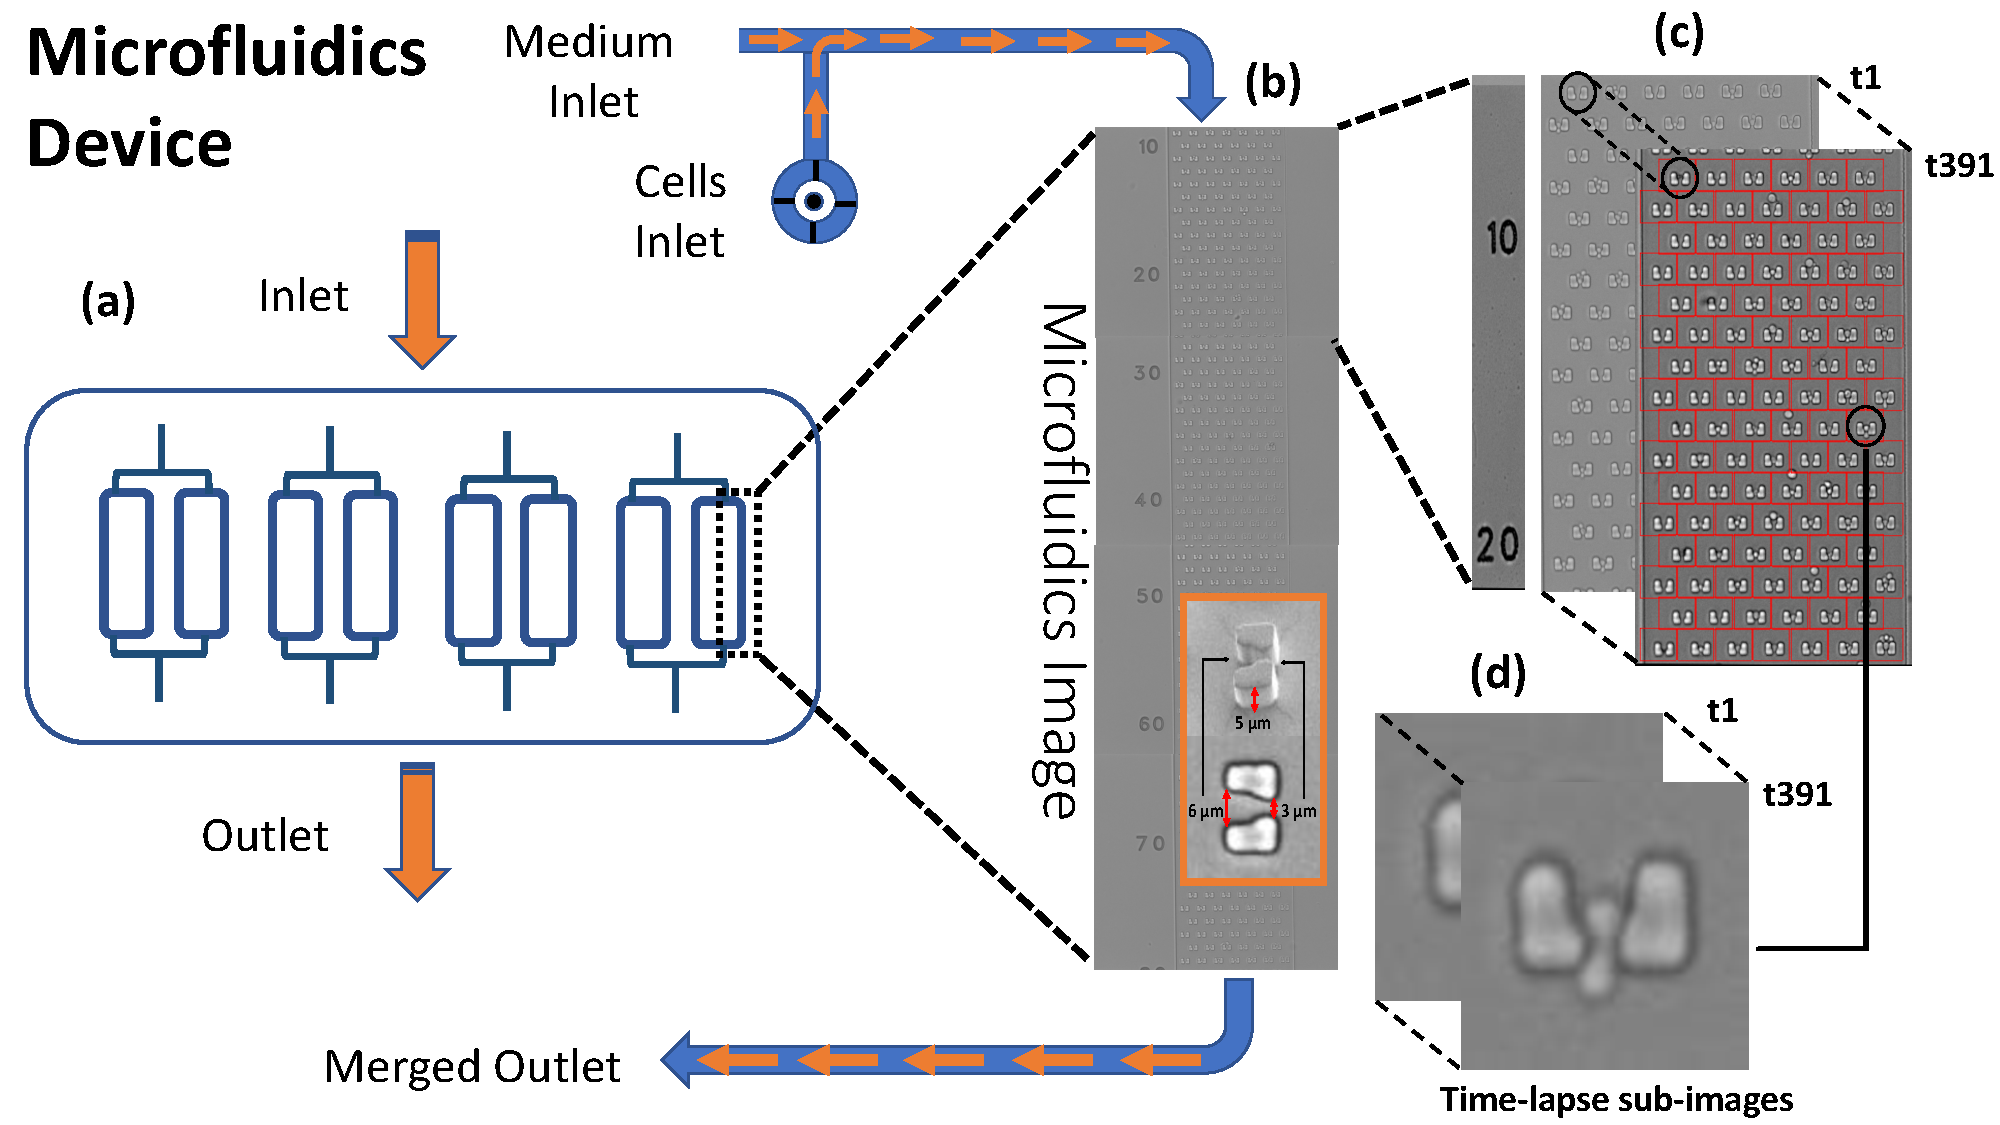
\includegraphics[width=\textwidth,height=10 cm]{Patterns/fluidics.pdf}
\caption{ HYAA microfluidics device with 16 channels. A time-point sample of microfludics image shown with guidelines 10 - 70. An  example of time-lapse images for guidelines 10 - 20  }
\label{fig:micro}
\end{figure*}

All time-lapse microfluidics images are captured with IX-81 Olympus inverted microscope equipped with an Olympus camera (DP72 CCD) operating by cellSens software. The experimental process took around 96 hours at a temperature of 86$^{\circ}$F (30$^{\circ}$C). Each channel has 520 traps inside the microfluidic chamber and each row has 7 or 6 traps consecutively. Channels are labeled with numbers right-side for capturing guidelines. The order of rows could be different depending on capturing adjustment. For instant, if the camera positioned on guidelines 10 and 20, the first row of the captured image starts with 7 traps and so on. The experiment ended with capturing 391 images with 10 minutes interval between images. 

\subsection{Data Pre-processing}
Since microfluidics images have relatively low resolution and are considered a challenging task for visualization, we partitioned every single image to sub-image based on the individual trap. Traps are labeled from time-point 1 to time-point 391 as illustrated in Fig.\ref{fig:micro}. All sub-images partitioned concerning local traps at 60x60 resolution. Images are captured at four locations of the microfluidics device. 1st position: camera covered guidelines 10-20. 2nd position: camera covered guidelines 30-40. 3rd position: camera covered guideline 50-60. 4th position: camera covered guideline 70. In this work, we have considered the dataset from 1st position as shown in Fig.\ref{fig:micro}. We used You Only Look Once (YOLOv3) \cite{ref20} machine learning model for image feature extraction. We collected 391 sequence sub-images for each trap, extract and label them as following: trap number (trap\_num),time number (time\_num), total number of cell (total\_objs), cell x coordinate (obj\_X), cell y coordinate(obj\_Y) and cell area (obj\_area) as shown in Fig.\ref{fig:table}. The features of each image are collected orderly by row and increases by the number of available objects in the image. For instance, the features of the first image input with four cells are collected by indicating four rows for each cell and assigning time number (time\_num) one for all of them. This labeling method continuously followed for the rest of the images.


\subsection{Distance calculation and time-points conversion}

The process of feature extraction carried on for 104 available traps as illustrated in Fig.\ref{fig:micro}. We then surcharged individual cell distance feature to the existing dataset by using the euclidean equation:

\begin{equation}
\begin{split}
d_i = \sqrt{(x_i -x_r)^2 + (y_i -y_r)^2}\\
\\
i =  [1,2,3,4,..., m ] \\
\\
\end{split}
\end{equation}

where $ d_i $ is distance between centroid point of cell and reference point. $ x_i $ and $ y_i $ are cells coordinate at each image. $ x_r $ and $ y_r $ are trap reference point. Generally, these points could be chosen at any point of image. We decided to choose the reference point based on cell flow direction and potential cell division point. $ i $ is image number corresponding to time-point and $ m $ is the maximum time-point equivalents to total number images. Here, $ x_r $ and  $ y_r $ are set to be 30 and 34 respectively at trap outlet as shown in $\nameref{S1_Fig}$. In further step, we converted time to degree by using: 
 
\begin{equation}
\begin{split}
 degree = \sum_{i=1}^{n}{theta_i}\\
 \\
\end{split}
\end{equation}

here, $theta $ = \text{maximum degree}$/$\text{maximum time} and $ degree $ is accumulative degree of each radius and $ n $ is equal to maximum degree(e.g, 360). All distance values are considered as radius for cell movement interpretation.     

\subsection{$\mu$Polar input}
Fig.\ref{fig:table} illustrates an example of traps at time-points 1 and 2. Time-point 1 shows distance between and area of each cell. dL1, dl2, dL3 and dL4 are distance from reference point. a1, a2, a3 and a4 are area of each cell. The table in Fig.\ref{fig:table} represents an example of the $\mu$Polar dataset format at two time-points. The dataset feature are labeled as following; trap\_num (trap number),  time\_num (image time number), total\_objs (total available cells inside image), obj\_X and obj\_Y are cell coordinate, area (cell area), dist (cell distance to reference point). Image at time-pint 1 belongs to rows 1 - 4 of table dedicating image with four cells and image at time-point 2 belongs to row 5 - 7 dedicating image with three cells. 


\begin{figure*}
\centering
\includegraphics[width=\textwidth,height=10 cm]{Patterns/table.pdf}
\caption{ A schematic and plot examples of $\mu$Polar.}
\label{fig:table}
\end{figure*}



\subsection{$\mu$Polar visualization paradigm}

Fig.\ref{fig:polar} shows a schematic of $\mu$Polar with some sample time-points for different trap. Images at time-points 1 - 5 are represented in $\mu$polar plot. The theta for time-points 1 - 5 are 0.92, 1.84, 2.76, 3.68, 4.6 respectively. The plot has two regions separated with red circle, denote as $ A $ region (above reference line) and $ B $ region ( below reference). In this example, cells in " orange " color are in $ A $  region and cells in "green" color are in $ B $ region. The cell size variation is based on cell area. The number of cell(s) on each time-point radius indicate the number cell (s) on the each image. For instance, there are two cells at time-point 1, three cells at time-point 2, three cells at time-point 3, two cells at time-point 4 and one cell at time-point 5 respectively. 

 
\begin{figure*}
\centering
\includegraphics[width=\textwidth,height=10 cm]{Patterns/polar.pdf}
\caption{ A schematic and plot examples of $\mu$Polar.}
\label{fig:polar}
\end{figure*}

\section{Discussion}
We developed an R package called "$\mu$Polar" for microfluidicss image visualization where any individual trap could be visualized based on number of cell and area. The package is using three libraries including "dplyr", "plyr" and "plotly". As shown in Fig.\ref{fig:table} the "$\mu$Polar" package requires image time number, total number of available cells in image and cell distance. The "$\mu$Polar" function takes dataset, time number, cell number, cell area, cell distance, offset value and total number of time. 

Fig.\ref{fig:polar} is an interpretation of a trap sequence images from time-point 1 to time-point 391. The color representation are based on number of available cell(s) in an image. Here, we used default setting where white color represents trap without cell, black color represents trap with one cell, green color represents trap with two cells, light-brown represents trap with 3 cells, blue color represents trap with 4 cells, orange color represents trap with 5 cells and sky-blue color represents trap with more than 5 cells. Furthermore, red circle color represents trap reference line. For instance , time-point 275 to  time-point 313 and time-point353 to time-point 360 are represented in white color and  laid on reference line (red). $ Tm  $ and  $ Ce $  are image time-point number and number of available cell(s) respectively. An An example of $\mu$Polar plot given at time-point 21 where cell color shown in black since there only single cell available.  

\subsection{$\mu$Polar cell area and offset}

Cell area and offset features could be used for better plot analysis. The cell area could be set to zero if the cell area information is not available. Furthermore, the offset value is to adjust the cap between maximum radius of dataset and plot out layer. These options could initially set to zero and change for better visualization. Fig.\ref{fig:areaoff}(a1) shows a $\mu$polar plot with cell area and offset are equaled to zero. In other word, the cell are set to 5 by default. Fig.\ref{fig:areaoff}(a2) shows $\mu$polar plot with offset value set to 8 where the gap between maximum radius and plot out layer increase by 8 units. Fig.\ref{fig:areaoff}(b1, b2) show $\mu$polar plot with cell area size decreased and increased by 2 and 8 units respectively. This option is useful for controlling over-size cells and monitoring cell dynamic shape, in particulate, if there is no division and cell reached its senescent stage.    

\begin{figure*}
\centering
\includegraphics[width=\textwidth,height=10 cm]{Patterns/area_offset.pdf}
\caption{ An example of time-lapse microfluidics images.}
\label{fig:areaoff}
\end{figure*}


\subsection{$\mu$Polar with RLS}

$\mu$Polar has addition option for replicative lifespan (RLS) visualization. This feature could be added to the plot if RLS dataset is available from dataset. The RLS division points appear inside plot out layer with "star" sign. we previously collected RLS data for there trap and applied these information for some $\mu$polar plot examples. Fig.\ref{fig:areaoff}(c1) shows $\mu$polar plot with countable red color "stat" representing  trap RLS. In this particular example, there are 22 red "stars" corresponding to the trap RLS. Fig.\ref{fig:areaoff}(c1) shows another  example of $\mu$polar plot with better cell division process. In this example, there are 13 red " stars" corresponding  to trap RLS.  
In order to have better visualization and avoid over lapping, it is advisable to chose offset value properly. Fig.\ref{fig:areaoff} shows an example of $\mu$Polar with RLS. The cell area and offset value set to zero and 10 respectively.        



\section{Stat * Method}

%example
% Mass cytometry experiments
% Mass cytometry data used in this manuscript, together with the information regarding cell preparation, data acquisition, and processing was obtained from the original publications (31-33). Through the rest of the manuscript, we will call these respective datasets by their main contributing authors: Bodenmiller/Zunder/Finck, Bendall/Davis/Amir, and Fragiadakis.





\section{Conclusion}


% \begin{figure*}
% \centering
% \includegraphics[width=\textwidth,height=10 cm]{Patterns/cellSteps.pdf}
% \caption{ An example of time-lapse microfluidics images.}
% \label{fig:imageData}
% \end{figure*}

\subsection{microfluidicss Device}
In the following, we summarize ... 
 
% \begin{figure*}
% \centering
% \includegraphics[width=\textwidth,height=10 cm]{Patterns/bc8_tp8.pdf}
% \caption{ An example of time-lapse microfluidics image (Beacon08 Trap08).}
% \label{fig:imageData}
% \end{figure*}


% \begin{figure*}
% \centering
% \includegraphics[width=\textwidth,height=10 cm]{Patterns/bc8_tp30.pdf}
% \caption{ An example of time-lapse microfluidics images (Beacon08 Trap30).}
% \label{fig:imageData}
% \end{figure*}


% \begin{figure*}
% \centering
% \includegraphics[width=\textwidth,height=10 cm]{Patterns/bc8_tp75.pdf}
% \caption{ An example of time-lapse microfluidics images (Beacon08 Trap75).}
% \label{fig:imageData}
% \end{figure*}


% \begin{figure*}
% \centering
% \includegraphics[width=\textwidth,height=10 cm]{Patterns/bc8_tp100.pdf}
% \caption{ An example of time-lapse microfluidics images (Beacon08 Trap100).}
% \label{fig:imageData}
% \end{figure*}


\section{Supplemental Information}

\paragraph*{S1 Fig.}
\label{S1_Fig}
{\bf  Cell distance calculation method.} (a) trap reference point. (b) an example of cell distance from reference point. (c) Sample of some images with labeled cells. 


\begin{figure*}
\centering
\includegraphics[width=\textwidth,height=10 cm]{Patterns/point.pdf}
\caption{ Examples of time-lapse microfluidics images.}
\label{fig:imageData}
\end{figure*} 



\paragraph*{S1 Table.}


\label{S1_Table}
{\bf Grid search and augmentation options.} A total of 108 combinations were trained without and with augmented dataset. 


\subsection*{Acknowledgment}

The work is partially supported by the NSF CAREER award \#1453078 (transferred to \#1720215), NSF award \#1761839, a  start-up fund, internal CEACSE awards from the University of Tennessee at Chattanooga, and the computing facility of the SimCenter at the University of Tennessee at Chattanooga. We also acknowledge the support of NIH grants \#R01AG052507 and \#R42AG058368.


\subsection*{Author contributions}


\subsection*{Declaration on interests}


\begin{thebibliography}{00}

\bibitem{r1}

CARPENTERA. E.: Image-based chemical screening.NatureChemical Biology 3, 8 (2007), 461–465


\bibitem{r2}
WOLLMANR., STUURMANN.: High throughput microscopy:From raw images to discoveries.Journal of Cell Science 120,21(2007), 3715–3722

\bibitem{r2.6}
Oates, A. C., Gorfinkiel, N., Gonzalez-Gaitan, M. & Heisenberg, C.-P. Quantitative approaches in developmental biology. Nat. Rev. Genet. 10, 517–530 (2009).



\bibitem{r2.7}
Amat, F. et al. Fast, accurate reconstruction of cell lineages from large-scale fluorescence microscopy data. Nat. Methods 11, 951–958 (2014).

\bibitem{r2.8}
Mavrakis, M., Rikhy, R., Lilly, M. & Lippincott-Schwartz, J. Fluorescence imaging techniques for studying Drosophila embryo development. Curr. Protoc. Cell Biol. 39, 4.18.1–4.18.43 (2008).

\bibitem{r2.9}
Buckingham, M. E. & Meilhac, S. M. Tracing cells for tracking cell lineage and clonal behavior. Dev. Cell 21, 394–409 (2011).

\bibitem{r2.10}
Olivier, N. et al. Cell lineage reconstruction of early zebrafish embryos using label-free nonlinear microscopy. Science 329, 967–971 (2010).


\bibitem{r2.2}
Farokhi H, Ghayesh MH (2018) Nonlinear mechanics of electrically actuated microplates. International Journal of Engineering Science 123: 197-213.

\bibitem{r2.1}
Ghayesh MH (2018) Mechanics of tapered AFG shear-deformable microbeams. Microsystem Technologies 24(4): 1743-1754.


\bibitem{r2.3}
Şimşek M (2016) Nonlinear free vibration of a functionally graded nanobeam using nonlocal strain gradient theory and a novel Hamiltonian approach. International Journal of Engineering Science 105: 12-27.

\bibitem{r2.4}
 Bhagat AAS, Bow H, Hou HW, Tan SJ, Han J, et al. (2010) Microfluidics for cell separation. Med Biol Eng Compu 48: 999-1014.

\bibitem{r2.5}
Shafiee H, Jahangir M, Inci F, Wang S, Willenbrecht RB, et al. (2013) Acute on-chip HIV detection through label-free electrical sensing of viral nano- lysate. Small 9(15): 2553-2563.




\bibitem{r3}
JENSENE. C.: Overview of live-cell imaging: Require-ments and methods used.The Anatomical Record 296, 1 (2013),1–8

\bibitem{ref01}

V. Longo, G. Shadel, M. Kaeberlein and B.  Kennedy, Replicative and Chronological Aging in Saccharomyces cerevisiae, Cell Metabolism, 2002,16(1):18-31.





\bibitem{ref02}
R. Eilsand and C. Athale, Computational imaging in cell biology, Cell Biol.2003, 16: 477-48.






\bibitem{ref03}
D. Webb and A. Horwitz, New dimensions in cell migration, Cell Biol, 2003,  5: 690-692.

% \bibitem{ref04}
% M. Kaeberlein, K. Kirkland, S. Fields and B. Kennedy, Sir2-Independent Life Span Extension by Calorie Restriction in Yeast, PLoS Biology,,2004, 2(9):e296.

\bibitem{ref4.2}
H. Qin, Estimating network changes from lifespan measurements using a parsimonious gene network model of cellular aging, BMC Bioinformatics 20, 599 ,2019, doi:10.1186/s12859-019-3177-7

% \bibitem{ref05}
%  R. Wilson et .al,Regulation of Yeast Replicative Life Span by TOR and Sch9 in Response to Nutrients. Science,2005, 310 : 1193-1196.

\bibitem{ref07}

D. Botstein and G. Fink, Yeast: An experimental organism for 21st Century biology. Genetics, 2001, 189(3): 695-704.


\bibitem{ref08}

K. Steffen, B. Kennedy and M Kaeberlein, Measuring replicative life span in the budding yeast, JoVE, 2009,  28: 1-5.

\bibitem{ref09}

M. Kaeberlein and B. Kennedy, Large-scale identification in yeast of conserved ageing genes. Mech Ageing Dev,2005, 126(1):17-21.

\bibitem{ref10}

D. Sinclair, K. Mills, and L. Guarente,  Aging in Saccharomyces cerevisiae, Annu. Rev,  Microbiol, 1998, 52: 533-560.


\bibitem{ref11}

S. Enfors  et al. , Physiological responses to mixing in large scale bioreactors, J Biotechnol,2001, 85: 175-185


\bibitem{ref12}

K. Chen, M. Crane and  M. Kaeberlein, microfluidics Technologies for Yeast Replicative Lifespan Studies. Mechanisms of ageing and development, 2017, 161(Pt B):262-269.


\bibitem{ref13}

 M. Jo, W. Liu, L. Gu, W. Dang and  L. Qin, High-throughput analysis of yeast replicative aging using a microfluidics system, Proc. Nati. Acad. Sci. USA, 2015, 112: 9364-9369.


\bibitem{ref14}

M. McCormick,  J.Delaney, M. Tsuchiya, et alA comprehensive analysis of replicative lifespan in 4,698 single-gene deletion strains uncovers conserved mechanisms of aging, Cell metabolism, 2015, 22(5):895-906.


\bibitem{ref15}
S. Pang,  et al. ,A novel YOLOv3-arch model for identifying cholelithiasis and classifying gallstones on CT images, PLoS ONE, 2019, 14(6): e0217647. https://doi.org/10.1371/journal. pone.021764

\bibitem{ref16}
C.  Laura, P. Hofmann, K. Drechselr  and S. Wesarg, Automatic detection of the nasal cavities and paranasal sinuses using deep neural networks, In IEEE 16th International Symposium on Biomedical Imaging,2019, pages 1154–1157. IEEE.

\bibitem{ref17}
J. Martin, et al., The impact of 2D cine MR imaging parameters on automated tumor and organ localization for MR-guided real-time adaptive radiotherapy. Physics in Medicine and Biology, 2018, 63(23):235005.

\bibitem{ref18}
S. Ramachandran, J. George, S. Skaria, and  V. Varun,  Using YOLO based deep learning network for real time detection and localization of lung nodules from low dose CT scans, In Kensaku Mori and Nicholas Petrick, editors, Medical Imaging 2018: Computer-Aided Diagnosis, 2018, volume 10575, page 53. SPIE.

\bibitem{ref19}
J. Redmon and A. Farhadi. YOLOv3: An Incremental Improvement. Technical report, University of Washington, 2018.

\bibitem{ref20}
Z. Zhao, P. Zheng, S. Xu, and X Wu, Object Detection With Deep Learning: A Review. IEEE Transactions on Neural Networks and Learning Systems, 2019, pages 1–21.


\end{thebibliography}



% We provide a concise description of live cell imaging in Section 
% 2. Next, in Section 
% 3, we describe our analytical approach. Based on this, Section 
% 4 contains the results of a systematic analysis of visualization methods cell imaging. 
% This includes reports on domain and data characterization (Section 4.1),
% task abstraction (Section 4.2), and
% visual encoding and interaction design (Section 4.3).
% We discuss the implications of our analysis,including a number of research gaps, in Section 5
% conclude with Section 6.


%https://www.osti.gov/servlets/purl/1557948
%https://onlinelibrary.wiley.com/doi/epdf/10.1111/cgf.12784



% Imaging of fluorescently labeled proteins in living cells provides spatial and temporal information on their subcellular localization. This is essential to understand their role in dynamic processes such as cell division. In addition, time-lapse microscopy allows direct analysis of the correlation (or lack thereof) between distinct events at the single cell level, which could be masked in bulk population studies such as time-courses of synchronized cultures. Such correlations might reveal functional relationships, coordination of events in space and time, and feedback regulatory loops (see [1] for a detailed discussion of these topics).
% In budding yeast cells, the site of cytokinesis (termed the bud neck) is marked by the presence of a membrane-associated, septin- based collar [2]. Cytokinesis begins at the end of mitosis when the septin collar splits into two rings, defining a compartment where actomyosin ring contraction takes place [3]. Closure of this con- tractile ring and septum deposition drive the overlying plasma membrane inward, in a process akin to furrow ingression in animal cells (see [4, 5] for reviews). The ring then disassembles, allowing fission of the contracted membrane, in a process termed abscission [3]. After completion of cytokinesis, cell wall degradation at the septation site allows separation of mother and daughter cells [6]. Here, we describe optimized methods to image multiple cytokinesis events in living yeast cells, namely septin ring dynamics, acto- myosin ring contraction, and plasma membrane ingression at the mother–bud neck.

% Time-lapse imaging files are relatively large and it is therefore useful to ensure that enough memory space and computer processing power are available to process them (each of the image fields in the above example represent 1200 [20×60] frames for each channel, between 0.5 and 1.5 GB in size).

%https://link.springer.com/content/pdf/10.1007%2F978-1-4939-3145-3.pdf














\end{document}
